\begin{figure}[t]
\centering
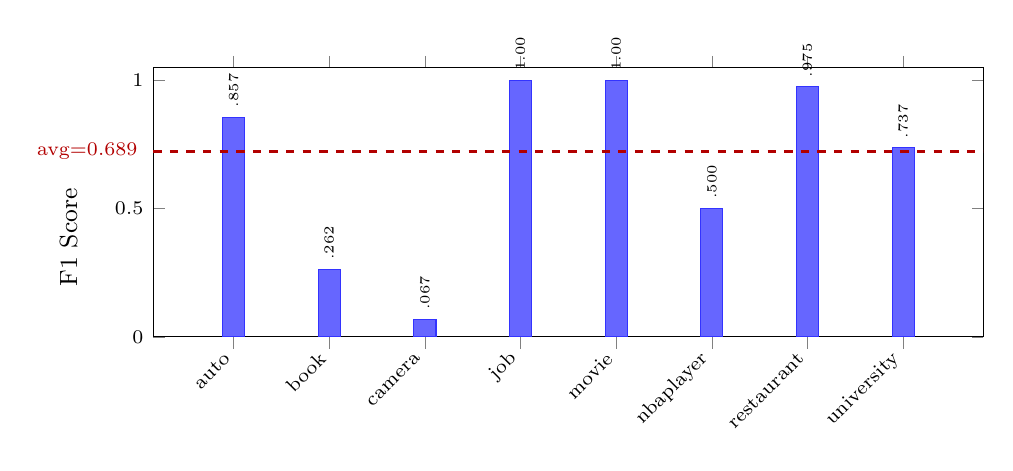
\begin{tikzpicture}
\begin{axis}[
  ybar,
  width=\columnwidth,
  height=5cm,
  bar width=8pt,
  ymin=0, ymax=1.05,
  ylabel={F1 Score},
  symbolic x coords={auto,book,camera,job,movie,nbaplayer,restaurant,university},
  xtick=data,
  x tick label style={rotate=45, anchor=east, font=\scriptsize},
  y tick label style={font=\scriptsize},
  ylabel style={font=\small, at={(axis description cs:-0.08,0.37)}},
  nodes near coords,
  every node near coord/.append style={font=\tiny, rotate=90, anchor=west},
  nodes near coords align={vertical},
  point meta=explicit symbolic,
  clip=false,
  enlarge x limits=0.12,
]
\addplot[fill=blue!60, draw=blue!80] coordinates {
  (auto,0.857) [.857]
  (book,0.262) [.262]
  (camera,0.067) [.067]
  (job,1.000) [1.00]
  (movie,1.000) [1.00]
  (nbaplayer,0.500) [.500]
  (restaurant,0.975) [.975]
  (university,0.737) [.737]
};
% Average line
\draw[dashed, thick, red!70!black] (rel axis cs:0,0.689) -- (rel axis cs:1,0.689)
  node[pos=0, anchor=east, font=\scriptsize, xshift=-2pt] {avg=0.689};
\end{axis}
\end{tikzpicture}
\caption{SWDEベンチマーク: バーティカル別F1スコア(検出フィールド)}
\ecaption{SWDE benchmark: F1 scores by vertical (found fields).}
\label{fig:swde}
\end{figure}
